\documentclass[11pt,a4paper]{article}
\usepackage[utf8]{inputenc}
\usepackage[french]{babel}
\usepackage[T1]{fontenc}
\usepackage{mathtools}
\usepackage{tikz}
\usepackage{amsmath, amssymb, amsthm}            
\usepackage{amstext, amsfonts, a4}
\usepackage{hyperref}
\usepackage[ruled,vlined, french, onelanguage]{algorithm2e}
\usepackage[left=2cm,right=2cm,top=2cm,bottom=2cm]{geometry}
\usepackage{multicol}
\usepackage{xcolor}
\usepackage{float}
\usepackage{lscape}


\def\ccB{\mathscr{B}}
\newcommand\numberthis{\addtocounter{equation}{1}\tag{\theequation}}


\begin{document}
%Cet algorithme est basé sur les développements de Taylor autour d'un point,
%de sorte que le Laplacien soit discrétisé comme suit :
%
%\section{Cas 1D}
%\begin{figure}[H]
%\centering
%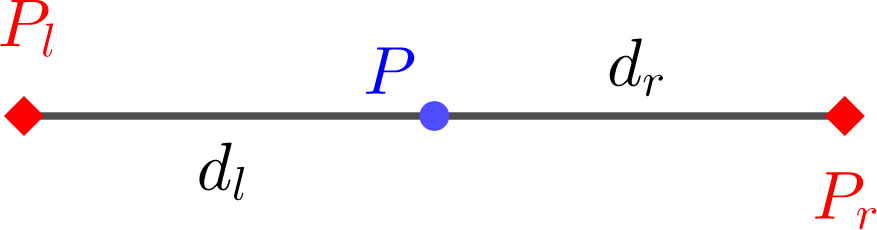
\includegraphics[width=0.3\textwidth]{export1D.png}
%\caption{Illustration 1D}
%\end{figure}
%
%\begin{equation*}
%[\Delta] u (P) = [\partial_x^2]u(P) \approx \frac{\frac{u(P_l) - u (P)}{d_l} - \frac{u(P) - u (P_r)}{d_r}}{\frac{d_r+d_l}{2}}
%\end{equation*}
%et donc que
%\begin{align*}
% u''(P)&\approx \frac{1}{\frac{d_l + d_r}{2}} \left( \frac{1}{d_l}\,u(P_l) - \left[\frac{1}{d_l} + \frac{1}{d_r}\right]\,u(P) + \frac{1}{d_r}\,u(P_r)\right)
%\end{align*}
%
%\section{Cas 2D}
%
%\begin{figure}[H]
%\centering
%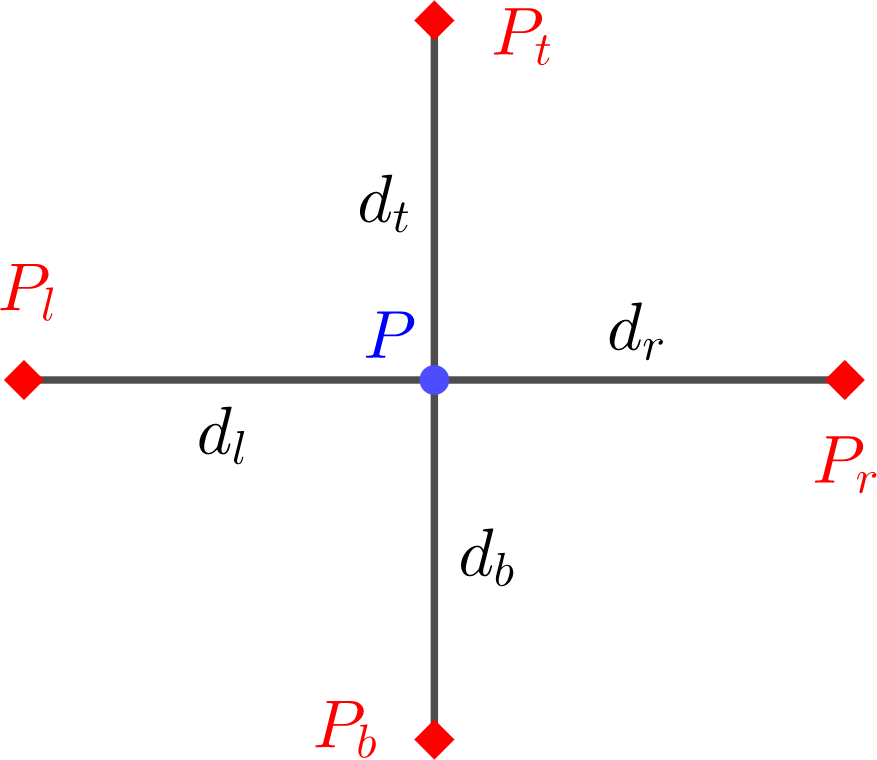
\includegraphics[width=0.3\textwidth]{export2D.png}
%\caption{Illustration 2D}
%\end{figure}
%
%\begin{align*}
%[\Delta] u (P) = [\partial_x^2 + \partial_y^2]u(P) &\approx \frac{\frac{u(P_l) - u (P)}{d_l} - \frac{u(P) - u (P_r)}{d_r}}{\frac{d_r+d_l}{2}}\\ 
%&+
%\frac{\frac{u(P_t) - u (P)}{d_t} - \frac{u(P) - u (P_b)}{d_b}}{\frac{d_t+d_b}{2}}
%\end{align*}
%et donc que
%\begin{align*}
%\Delta u (P)&\approx \frac{1}{\frac{d_l + d_r}{2}} \left( \frac{1}{d_l}\,u(P_l) - \left[\frac{1}{d_l} + \frac{1}{d_r}\right]\,u(P) + \frac{1}{d_r}\,u(P_r)\right) \\
%&+
%\frac{1}{\frac{d_t + d_b}{2}} \left(\frac{1}{d_t}\,u(P_t) - \left[\frac{1}{d_t} + \frac{1}{d_b}\right]\,u(P) + \frac{1}{d_b}\,u(P_b)\right) 
%\end{align*}
%
%\section{Cas 3D}
%
%\begin{figure}[H]
%\centering
%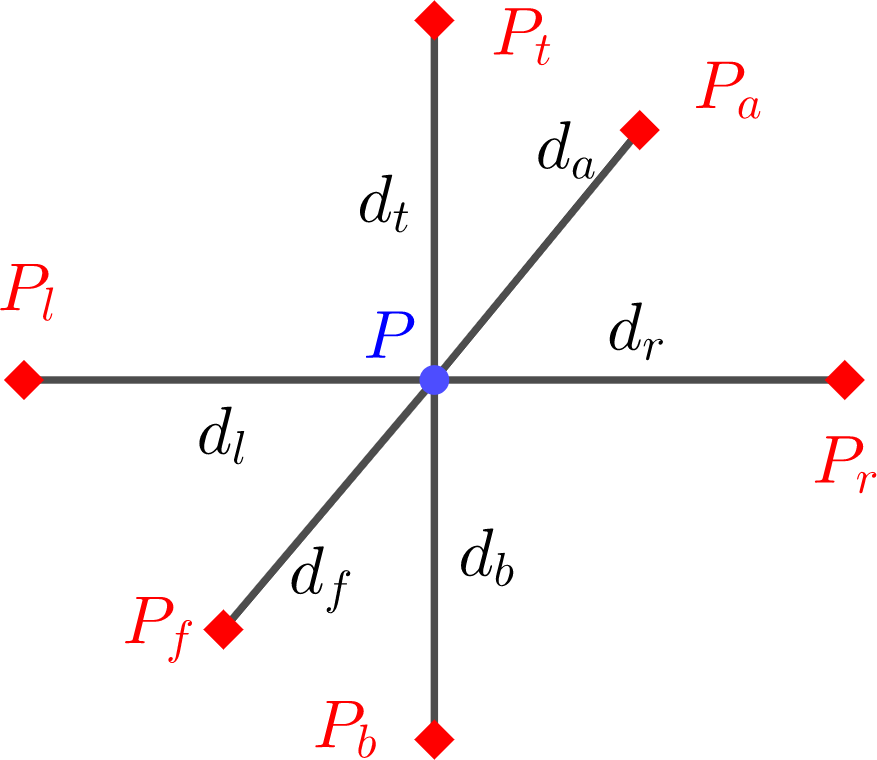
\includegraphics[width=0.3\textwidth]{export3D.png}
%\caption{Illustration 3D}
%\end{figure}
%
%\begin{align*}
%[\Delta] u (P) = [\partial_x^2 + \partial_y^2 + \partial_z^2]u(P) &\approx \frac{\frac{u(P_l) - u (P)}{d_l} - \frac{u(P) - u (P_r)}{d_r}}{\frac{d_r+d_l}{2}} \\
%&+
%\frac{\frac{u(P_t) - u (P)}{d_t} - \frac{u(P) - u (P_b)}{d_b}}{\frac{d_t+d_b}{2}}\\
%&+
%\frac{\frac{u(P_f) - u (P)}{d_f} - \frac{u(P) - u (P_a)}{d_a}}{\frac{d_f+d_a}{2}}
%\end{align*}
%et donc que
%\begin{align*}
% \Delta u (P)&\approx \frac{1}{\frac{d_l + d_r}{2}} \left( \frac{1}{d_l}\,u(P_l) - \left[\frac{1}{d_l} + \frac{1}{d_r}\right]\,u(P) + \frac{1}{d_r}\,u(P_r)\right) \\
%&+
%\frac{1}{\frac{d_t + d_b}{2}} \left(\frac{1}{d_t}\,u(P_t) - \left[\frac{1}{d_t} + \frac{1}{d_b}\right]\,u(P) + \frac{1}{d_b}\,u(P_b)\right) \\
%&+
%\frac{1}{\frac{d_f + d_a}{2}} \left(\frac{1}{d_f}\,u(P_f) - \left[\frac{1}{d_f} + \frac{1}{d_a}\right]\,u(P) + \frac{1}{d_a}\,u(P_a)\right) 
%\end{align*}

%\newpage
\begin{algorithm}[H]
\SetAlgoLined
Soit $A:=\left(\begin{array}{c|c}
M & 0\\
\hline
0 & 0
\end{array}\right)$\\
~\\
\ForEach{$p_k$ : points du bord}
{
	\textbf{$p_k$ : le point de bord considéré d'indice global $k$}\\
	~\\
	\If{$p_k$ est un point du maillage} 
	{	
		\textcolor{red}{\textbf{On passe au point $p_k$ suivant}}\\
	}
	~\\
	\textbf{$p_l$ : premier voisin de $p_k$ d'indice global $l$}\\
	\textbf{$p_r$ : deuxième voisin de $p_k$ d'indice global $r$}\\
	~\\
	\textbf{$\gamma$ : axe sur lequel est placé l'arête $[p_l,p_r]$ (ie soit $x$ ou $y$ ou $z$)}\\
	~\\
	\textcolor{red}{\textbf{Nous devons dans un premier temps les interactions entre $p_l$ et $p_r$ :}}
	\begin{center}
	$A [l, r] = A [r, l] = 0$
	\end{center}
	\textcolor{red}{\textbf{Il nous faut ensuite actualiser la ligne $k$ :}}
	\begin{center}
	$A [k, :] = 0$\hspace{1cm}\textbf{Actualise\_ligne $(k, \gamma)$}
	\end{center}
	\textcolor{red}{\textbf{Et il nous faut actualiser les lignes $l$ et $r$ :}}
	\begin{center}
	\textbf{Actualise\_ligne $(l, \gamma)$}\hspace{1cm}
	\textbf{Actualise\_ligne $(r, \gamma)$}
	\end{center}
}
\caption{Insertion de coefficients dans la matrice}
\end{algorithm}

\begin{algorithm}[H]
\SetAlgoLined
~\\
\textbf{$p_m$ : le point considéré d'indice global $m$}\\
~\\

\textbf{$p_l$ : voisin de $p_m$ dans la direction $(-\gamma)$ d'indice global de $l$}\\
\textbf{$p_r$ : voisin de $p_m$ dans la direction $(+\gamma)$ d'indice global de $r$}\\
~\\
$d_r$ : distance entre $p_r$ et $p_m$\\
$d_l$ : distance entre $p_m$ et $p_l$\\
~\\
$moy = \frac{d_l + d_r}{2}$\\
~\\
\textcolor{red}{\textbf{Calculons l'interaction entre $m$ et $l$ :}}
\begin{center}
$A [m, l] = - \frac{D}{moy} \times \frac{1}{d_l}$
\end{center}
\textcolor{red}{\textbf{Calculons l'interaction entre $m$ et $r$ :}}
\begin{center}
$A [m, r] = - \frac{D}{moy} \times \frac{1}{d_r}$
\end{center}
\textcolor{red}{\textbf{Écrasons temporairement le coefficient diagonal :}}
\begin{center}
$A[m,m] = 0$
\end{center}
\textcolor{red}{\textbf{Sommons la ligne $m$ pour avoir le coefficient diagonal :}}
\begin{center}
$A[m,m] = -\sum_{i=0}^{N}\,A[m, i]$
\end{center}

\caption{\textbf{Actualise\_ligne (Entier $m$, axe\_arête $\gamma$)}}
\end{algorithm}

\newpage
\newgeometry{paper= a3paper}

\begin{landscape}
\begin{equation}
\left(\begin{array}{cccccccccccccccccc} \frac{1}{\mathrm{dt}}+\frac{2\,{\mathrm{dx}}^2}{D}+\frac{2\,{\mathrm{dy}}^2}{D} & -\frac{{\mathrm{dx}}^2}{D} & 0 & 0 & -\frac{{\mathrm{dy}}^2}{D} & 0 & 0 & 0 & -\frac{{\mathrm{dy}}^2}{D} & 0 & 0 & -\frac{{\mathrm{dx}}^2}{D} & 0 & 0 & 0 & 0 & 0 & 0\\ -\frac{{\mathrm{dx}}^2}{D} & \frac{2\,{\mathrm{dx}}^2}{D}+\frac{D}{{\mathrm{dx}}^2\,\left(\frac{{\mathrm{dx}}^2}{2}+\frac{\mathrm{dy}}{2}\right)}+\frac{D}{\mathrm{dy}\,\left(\frac{{\mathrm{dx}}^2}{2}+\frac{\mathrm{dy}}{2}\right)} & -\frac{{\mathrm{dx}}^2}{D} & 0 & 0 & 0 & 0 & 0 & 0 & -\frac{D}{\mathrm{dy}\,\left(\frac{{\mathrm{dx}}^2}{2}+\frac{\mathrm{dy}}{2}\right)} & 0 & 0 & -\frac{D}{{\mathrm{dx}}^2\,\left(\frac{{\mathrm{dx}}^2}{2}+\frac{\mathrm{dy}}{2}\right)} & 0 & 0 & 0 & 0 & 0\\ 0 & -\frac{{\mathrm{dx}}^2}{D} & \frac{2\,{\mathrm{dx}}^2}{D}+\frac{D}{4\,{\mathrm{dx}}^2\,\left(2\,{\mathrm{dx}}^2+\frac{\mathrm{dy}}{2}\right)}+\frac{D}{\mathrm{dy}\,\left(2\,{\mathrm{dx}}^2+\frac{\mathrm{dy}}{2}\right)} & -\frac{{\mathrm{dx}}^2}{D} & 0 & 0 & 0 & 0 & 0 & 0 & -\frac{D}{\mathrm{dy}\,\left(2\,{\mathrm{dx}}^2+\frac{\mathrm{dy}}{2}\right)} & 0 & 0 & -\frac{D}{4\,{\mathrm{dx}}^2\,\left(2\,{\mathrm{dx}}^2+\frac{\mathrm{dy}}{2}\right)} & 0 & 0 & 0 & 0\\ 0 & 0 & -\frac{{\mathrm{dx}}^2}{D} & \frac{1}{\mathrm{dt}}+\frac{2\,{\mathrm{dx}}^2}{D}+\frac{2\,{\mathrm{dy}}^2}{D} & -\frac{{\mathrm{dx}}^2}{D} & 0 & 0 & -\frac{{\mathrm{dy}}^2}{D} & 0 & 0 & 0 & -\frac{{\mathrm{dy}}^2}{D} & 0 & 0 & 0 & 0 & 0 & 0\\ -\frac{{\mathrm{dy}}^2}{D} & 0 & 0 & -\frac{{\mathrm{dx}}^2}{D} & \frac{1}{\mathrm{dt}}+\frac{2\,{\mathrm{dx}}^2}{D}+\frac{2\,{\mathrm{dy}}^2}{D} & -\frac{{\mathrm{dx}}^2}{D} & 0 & 0 & -\frac{{\mathrm{dy}}^2}{D} & 0 & 0 & 0 & 0 & 0 & 0 & 0 & 0 & 0\\ 0 & -\frac{{\mathrm{dy}}^2}{D} & 0 & 0 & -\frac{{\mathrm{dx}}^2}{D} & \frac{2\,D}{{\left(\mathrm{dx}-\mathrm{dy}\right)}^4}+\frac{2\,{\mathrm{dx}}^2}{D}+\frac{{\mathrm{dy}}^2}{D} & -\frac{{\mathrm{dx}}^2}{D} & 0 & 0 & 0 & 0 & 0 & -\frac{D}{{\left(\mathrm{dx}-\mathrm{dy}\right)}^4} & 0 & 0 & -\frac{D}{{\left(\mathrm{dx}-\mathrm{dy}\right)}^4} & 0 & 0\\ 0 & 0 & -\frac{{\mathrm{dy}}^2}{D} & 0 & 0 & -\frac{D}{{\left(\mathrm{dx}-\mathrm{dy}\right)}^2\,\left(\frac{{\left(d_{5}+2\,\mathrm{dx}-\mathrm{dy}\right)}^2}{2}+\frac{{\left(\mathrm{dx}-\mathrm{dy}\right)}^2}{2}\right)} & \frac{{\mathrm{dy}}^2}{D}+\frac{2\,D}{{\left(2\,\mathrm{dx}-\mathrm{dy}\right)}^4}+\frac{D}{\left(\frac{{\left(d_{5}+2\,\mathrm{dx}-\mathrm{dy}\right)}^2}{2}+\frac{{\left(\mathrm{dx}-\mathrm{dy}\right)}^2}{2}\right)\,{\left(d_{5}+2\,\mathrm{dx}-\mathrm{dy}\right)}^2}+\frac{D}{{\left(\mathrm{dx}-\mathrm{dy}\right)}^2\,\left(\frac{{\left(d_{5}+2\,\mathrm{dx}-\mathrm{dy}\right)}^2}{2}+\frac{{\left(\mathrm{dx}-\mathrm{dy}\right)}^2}{2}\right)} & 0 & 0 & 0 & 0 & 0 & 0 & -\frac{D}{{\left(2\,\mathrm{dx}-\mathrm{dy}\right)}^4} & 0 & 0 & -\frac{D}{\left(\frac{{\left(d_{5}+2\,\mathrm{dx}-\mathrm{dy}\right)}^2}{2}+\frac{{\left(\mathrm{dx}-\mathrm{dy}\right)}^2}{2}\right)\,{\left(d_{5}+2\,\mathrm{dx}-\mathrm{dy}\right)}^2} & -\frac{D}{{\left(2\,\mathrm{dx}-\mathrm{dy}\right)}^4}\\ 0 & 0 & 0 & -\frac{{\mathrm{dy}}^2}{D} & -\frac{D}{\mathrm{dx}\,\left(\frac{\mathrm{dx}}{2}+\frac{{\left(d_{5}+2\,\mathrm{dx}-\mathrm{dy}\right)}^2}{2}\right)} & 0 & -\frac{{\mathrm{dx}}^2}{D} & \frac{2\,{\mathrm{dx}}^2}{D}+\frac{2\,{\mathrm{dy}}^2}{D}+\frac{D}{\left(\frac{\mathrm{dx}}{2}+\frac{{\left(d_{5}+2\,\mathrm{dx}-\mathrm{dy}\right)}^2}{2}\right)\,{\left(d_{5}+2\,\mathrm{dx}-\mathrm{dy}\right)}^2}+\frac{D}{\mathrm{dx}\,\left(\frac{\mathrm{dx}}{2}+\frac{{\left(d_{5}+2\,\mathrm{dx}-\mathrm{dy}\right)}^2}{2}\right)} & -\frac{{\mathrm{dx}}^2}{D} & 0 & 0 & -\frac{{\mathrm{dy}}^2}{D} & 0 & 0 & 0 & 0 & -\frac{D}{\left(\frac{\mathrm{dx}}{2}+\frac{{\left(d_{5}+2\,\mathrm{dx}-\mathrm{dy}\right)}^2}{2}\right)\,{\left(d_{5}+2\,\mathrm{dx}-\mathrm{dy}\right)}^2} & 0\\ -\frac{{\mathrm{dy}}^2}{D} & 0 & 0 & 0 & -\frac{{\mathrm{dy}}^2}{D} & 0 & 0 & -\frac{{\mathrm{dx}}^2}{D} & \frac{1}{\mathrm{dt}}+\frac{2\,{\mathrm{dx}}^2}{D}+\frac{2\,{\mathrm{dy}}^2}{D} & -\frac{{\mathrm{dx}}^2}{D} & 0 & 0 & 0 & 0 & 0 & 0 & 0 & 0\\ 0 & -\frac{D}{\mathrm{dy}\,\left(\frac{\mathrm{dy}}{2}+\frac{{\left(\mathrm{dx}-2\,\mathrm{dy}\right)}^2}{2}\right)} & 0 & 0 & 0 & -\frac{{\mathrm{dy}}^2}{D} & 0 & 0 & -\frac{{\mathrm{dx}}^2}{D} & \frac{2\,{\mathrm{dx}}^2}{D}+\frac{{\mathrm{dy}}^2}{D}+\frac{D}{\mathrm{dy}\,\left(\frac{\mathrm{dy}}{2}+\frac{{\left(\mathrm{dx}-2\,\mathrm{dy}\right)}^2}{2}\right)}+\frac{D}{\left(\frac{\mathrm{dy}}{2}+\frac{{\left(\mathrm{dx}-2\,\mathrm{dy}\right)}^2}{2}\right)\,{\left(\mathrm{dx}-2\,\mathrm{dy}\right)}^2} & -\frac{{\mathrm{dx}}^2}{D} & 0 & 0 & 0 & 0 & -\frac{D}{\left(\frac{\mathrm{dy}}{2}+\frac{{\left(\mathrm{dx}-2\,\mathrm{dy}\right)}^2}{2}\right)\,{\left(\mathrm{dx}-2\,\mathrm{dy}\right)}^2} & 0 & 0\\ 0 & 0 & -\frac{D}{\mathrm{dy}\,\left(\frac{\mathrm{dy}}{2}+\frac{{\left(2\,\mathrm{dx}-2\,\mathrm{dy}\right)}^2}{2}\right)} & 0 & 0 & 0 & -\frac{{\mathrm{dy}}^2}{D} & 0 & 0 & -\frac{{\mathrm{dx}}^2}{D} & \frac{2\,{\mathrm{dx}}^2}{D}+\frac{{\mathrm{dy}}^2}{D}+\frac{D}{\left(\frac{\mathrm{dy}}{2}+\frac{{\left(2\,\mathrm{dx}-2\,\mathrm{dy}\right)}^2}{2}\right)\,{\left(2\,\mathrm{dx}-2\,\mathrm{dy}\right)}^2}+\frac{D}{\mathrm{dy}\,\left(\frac{\mathrm{dy}}{2}+\frac{{\left(2\,\mathrm{dx}-2\,\mathrm{dy}\right)}^2}{2}\right)} & -\frac{{\mathrm{dx}}^2}{D} & 0 & 0 & 0 & 0 & 0 & -\frac{D}{\left(\frac{\mathrm{dy}}{2}+\frac{{\left(2\,\mathrm{dx}-2\,\mathrm{dy}\right)}^2}{2}\right)\,{\left(2\,\mathrm{dx}-2\,\mathrm{dy}\right)}^2}\\ -\frac{{\mathrm{dx}}^2}{D} & 0 & 0 & -\frac{{\mathrm{dy}}^2}{D} & 0 & 0 & 0 & -\frac{{\mathrm{dy}}^2}{D} & 0 & 0 & -\frac{{\mathrm{dx}}^2}{D} & \frac{1}{\mathrm{dt}}+\frac{2\,{\mathrm{dx}}^2}{D}+\frac{2\,{\mathrm{dy}}^2}{D} & 0 & 0 & 0 & 0 & 0 & 0\\ 0 & -\frac{D}{{\left(d_{1}-\mathrm{dx}\right)}^4} & 0 & 0 & 0 & -\frac{D}{{\left(d_{1}-\mathrm{dx}\right)}^4} & 0 & 0 & 0 & 0 & 0 & 0 & \frac{2\,D}{{\left(d_{1}-\mathrm{dx}\right)}^4} & 0 & 0 & 0 & 0 & 0\\ 0 & 0 & -\frac{D}{{\left(d_{2}-2\,\mathrm{dx}\right)}^4} & 0 & 0 & 0 & -\frac{D}{{\left(d_{2}-2\,\mathrm{dx}\right)}^4} & 0 & 0 & 0 & 0 & 0 & 0 & \frac{2\,D}{{\left(d_{2}-2\,\mathrm{dx}\right)}^4} & 0 & 0 & 0 & 0\\ 0 & 0 & 0 & 0 & 0 & 0 & 0 & 0 & 0 & 0 & 0 & 0 & 0 & 0 & 0 & 0 & 0 & 0\\ 0 & 0 & 0 & 0 & 0 & -\frac{D}{{\left(d_{4}-\mathrm{dx}+\mathrm{dy}\right)}^4} & 0 & 0 & 0 & -\frac{D}{{\left(d_{4}-\mathrm{dx}+\mathrm{dy}\right)}^4} & 0 & 0 & 0 & 0 & 0 & \frac{2\,D}{{\left(d_{4}-\mathrm{dx}+\mathrm{dy}\right)}^4} & 0 & 0\\ 0 & 0 & 0 & 0 & 0 & 0 & -\frac{D}{\left(\frac{{\left(2\,\mathrm{dx}-\mathrm{dy}\right)}^2}{2}+\frac{{\left(3\,\mathrm{dx}-\mathrm{dy}\right)}^2}{2}\right)\,{\left(2\,\mathrm{dx}-\mathrm{dy}\right)}^2} & -\frac{D}{\left(\frac{{\left(2\,\mathrm{dx}-\mathrm{dy}\right)}^2}{2}+\frac{{\left(3\,\mathrm{dx}-\mathrm{dy}\right)}^2}{2}\right)\,{\left(3\,\mathrm{dx}-\mathrm{dy}\right)}^2} & 0 & 0 & 0 & 0 & 0 & 0 & 0 & 0 & \frac{D}{\left(\frac{{\left(2\,\mathrm{dx}-\mathrm{dy}\right)}^2}{2}+\frac{{\left(3\,\mathrm{dx}-\mathrm{dy}\right)}^2}{2}\right)\,{\left(2\,\mathrm{dx}-\mathrm{dy}\right)}^2}+\frac{D}{\left(\frac{{\left(2\,\mathrm{dx}-\mathrm{dy}\right)}^2}{2}+\frac{{\left(3\,\mathrm{dx}-\mathrm{dy}\right)}^2}{2}\right)\,{\left(3\,\mathrm{dx}-\mathrm{dy}\right)}^2} & 0\\ 0 & 0 & 0 & 0 & 0 & 0 & -\frac{D}{{\left(d_{6}-2\,\mathrm{dx}+\mathrm{dy}\right)}^4} & 0 & 0 & 0 & -\frac{D}{{\left(d_{6}-2\,\mathrm{dx}+\mathrm{dy}\right)}^4} & 0 & 0 & 0 & 0 & 0 & 0 & \frac{2\,D}{{\left(d_{6}-2\,\mathrm{dx}+\mathrm{dy}\right)}^4} \end{array}\right)
\end{equation}
\end{landscape}
\restoregeometry
\newpage
\end{document}